\documentclass[aspectratio=169,11pt]{beamer}
\usepackage[utf8]{inputenc}
\DeclareUnicodeCharacter{21D2}{$\Rightarrow$}
\DeclareUnicodeCharacter{21A6}{$\mapsto$}
\DeclareUnicodeCharacter{2080}{$_0$}
\DeclareUnicodeCharacter{03B3}{$\gamma$}
\DeclareUnicodeCharacter{03BA}{$\kappa$}
\DeclareUnicodeCharacter{03C3}{$\sigma$}
\DeclareUnicodeCharacter{03C9}{$\omega$}
\DeclareUnicodeCharacter{03BC}{$\mu$}
\DeclareUnicodeCharacter{03C1}{$\rho$}
\DeclareUnicodeCharacter{03B9}{$\iota$}
\DeclareUnicodeCharacter{03B5}{$\varepsilon$}
\DeclareUnicodeCharacter{03C4}{$\tau$}
\DeclareUnicodeCharacter{0394}{$\Delta$}
\DeclareUnicodeCharacter{2264}{$\leq$}
\DeclareUnicodeCharacter{2265}{$\geq$}
\DeclareUnicodeCharacter{2260}{$\neq$}
\DeclareUnicodeCharacter{2205}{$\emptyset$}
\DeclareUnicodeCharacter{2192}{$\to$}
\DeclareUnicodeCharacter{211D}{$\mathbb{R}$}
\DeclareUnicodeCharacter{2115}{$\mathbb{N}$}
\DeclareUnicodeCharacter{207B}{$^{-}$}
\DeclareUnicodeCharacter{00B9}{$^{1}$}
\usepackage[T1]{fontenc}
\usepackage[english]{babel}
\usepackage{amsmath,amssymb}
\usepackage{booktabs}
\usepackage{graphicx}
\usepackage{listings}
\usetheme{default}
\usecolortheme{seahorse}
\setbeamertemplate{navigation symbols}{}
\setbeamertemplate{footline}[frame number]
\setbeamerfont{frametitle}{size=\large}

\lstdefinelanguage{Lean}{
  morekeywords={theorem,lemma,def,noncomputable,by,intro,apply,exact,have,rw,simp,only,
    linarith,nlinarith,omega,show,fun,let,if,then,else,Prop,Type,Finset,Monotone,Antitone,
    refine,change,rcases,obtain,set,with,at,change,HasDerivAt,StrictAntiOn,StrictMonoOn,
    AntitoneOn,MonotoneOn,ContinuousOn},
  sensitive=true,
  morecomment=[l]{--},
  morecomment=[s]{/-}{-/},
}
\lstset{
  language=Lean,
  basicstyle=\ttfamily\scriptsize,
  keywordstyle=\color{blue!70!black}\bfseries,
  commentstyle=\color{gray},
  columns=fullflexible,
  keepspaces=true,
  breaklines=true,
  extendedchars=true,
  inputencoding=utf8,
  literate=
    {∀}{{$\forall$}}1 {∃}{{$\exists$}}1 {ι}{{$\iota$}}1 {ℝ}{{$\mathbb{R}$}}1 {ℕ}{{$\mathbb{N}$}}1
    {→}{{$\to$}}1 {↔}{{$\leftrightarrow$}}1 {∑}{{$\sum$}}1 {∈}{{$\in$}}1
    {≤}{{$\leq$}}1 {≥}{{$\geq$}}1 {≠}{{$\neq$}}1 {⟨}{{$\langle$}}1 {⟩}{{$\rangle$}}1
    {₀}{{$_0$}}1 {Δ}{{$\Delta$}}1 {ω}{{$\omega$}}1 {σ}{{$\sigma$}}1 {ρ}{{$\rho$}}1
    {γ}{{$\gamma$}}1 {κ}{{$\kappa$}}1 {μ}{{$\mu$}}1 {¬}{{$\neg$}}1 {∧}{{$\wedge$}}1
    {·}{{$\cdot$}}1 {Ω}{{$\Omega$}}1 {⇒}{{$\Rightarrow$}}1 {↦}{{$\mapsto$}}1
    {∅}{{$\emptyset$}}1 {χ}{{$\chi$}}1 {ψ}{{$\psi$}}1 {η}{{$\eta$}}1 {ν}{{$\nu$}}1
    {θ}{{$\theta$}}1 {←}{{$\leftarrow$}}1 {ε}{{$\varepsilon$}}1 {τ}{{$\tau$}}1
    {⁻¹}{{$^{-1}$}}2
}

\newcommand{\ind}{\mathbf 1}

\title{Acemoglu, Kong \& Ozdaglar (2026)}
\subtitle{\emph{AI, Human Cognition and Knowledge Collapse} --- the static problem, Observation 1, and what Lean says about it}
\author{Manuel Arriola}
\date{Repository 4 \textperiodcentered{} Week of September 7 -- 12, 2026}

\begin{document}

%================= PORTADA =============================================
\begin{frame}[plain]
  \titlepage
  \begin{center}\small
    \texttt{github.com/Arriola123456/ai-04-acemoglu}\\[2pt]
    \footnotesize Version read: MIT working paper dated May 5, 2026 (NBER WP 34910, issued February 2026); backup slides after slide 4.
  \end{center}
\end{frame}

%================= 1. EL PAPER Y EL PROBLEMA =========================
\begin{frame}{1 \textperiodcentered{} The paper and the agent's problem}
  \footnotesize
  \textbf{Question.} Agentic AI gives each person accurate \emph{context-specific} advice. Does it erode the
  \emph{general} knowledge that makes context-specific information useful --- and can a society lose it?

  \smallskip
  \textbf{Primitives (Section 3.1).} A common state $\theta_t$ (random walk; general knowledge) and an
  idiosyncratic state $\theta_{i,t}$ (own context). Output $f(\ind\{|x-\theta_t|\le 1\},\ind\{|y-\theta_{i,t}|\le 1\})$
  with $\Delta_G=f(1,0)-f(0,0)$, $\Delta_I=f(0,1)-f(0,0)$, $\Delta_X=f(1,1)-f(1,0)-f(0,1)+f(0,0)$.
  \textbf{Assumption 1:} $\Delta_I=0$, $\Delta_X>0$ --- context is worthless without general knowledge.

  \smallskip
  \textbf{Learning.} Effort $e$ costs $\tfrac{\varepsilon}{\varepsilon+1}e^{(\varepsilon+1)/\varepsilon}$ and buys a
  private signal on own context (precision $\lambda_I e$) \emph{and} a thin public signal on $\theta_t$ pooled
  into the community's stock (precision $\lambda_G E$, an externality). Agentic AI adds a signal on own context
  with precision $\tau_A$. Posterior precisions: public $X_t$; idiosyncratic $Y=\sigma^{-2}+\lambda_I e+\tau_A$.

  \textbf{The agent's problem} (posterior-mean predictions; $G(\tau)=2\Phi(\sqrt\tau)-1$, $g=G'$):
  \vspace{-4pt}
  \[
    \max_{e\ge 0}\ U=f(0,0)+G(X)\Delta_G+G(X)G(Y)\Delta_X-\tfrac{\varepsilon}{\varepsilon+1}e^{\frac{\varepsilon+1}{\varepsilon}},
    \qquad
    \frac{\partial U}{\partial e}=\Delta_X G(X)\lambda_I g(Y)-e^{1/\varepsilon}=0 .
  \]
  \vspace{-6pt}
  She internalises only her own context; the general knowledge she creates is an externality.
\end{frame}

%================= 2. RESULTADO PRINCIPAL =============================
\begin{frame}{2 \textperiodcentered{} The main result, with all its conditions}
  \footnotesize
  \textbf{Observation 1 (Section 3.4).} \emph{Public precision $X_t$ complements human effort, while agentic-AI
  precision $\tau_A$ substitutes for it:}
  \[
    \frac{\partial^2 U}{\partial e\,\partial X}=\Delta_X\lambda_I\,g(X)\,g(Y)>0,
    \qquad
    \frac{\partial^2 U}{\partial e\,\partial\tau_A}=\Delta_X G(X)\lambda_I\,g'(Y)<0 .
  \]
  \begin{itemize}
    \item[(i)] \textbf{Assumption 1:} $\Delta_I=0$ (the private return to effort runs \emph{entirely} through
      $G(X)G(Y)\Delta_X$) and $\Delta_X>0$.
    \item[(ii)] $\lambda_I>0$; $X>0$ so that $G(X)>0$ (at $X=0$ effort is worthless: footnote 6).
    \item[(iii)] Gaussian facts: $G'=g>0$ and $g'<0$ --- diminishing returns to precision; $g(\tau)=\varphi(\sqrt\tau)/\sqrt\tau$.
    \item[(iv)] Additive precision $Y=\sigma^{-2}+\lambda_I e+\tau_A$: the AI signal and own learning are
      \emph{perfect substitutes} in producing context-specific precision (Equation 4).
    \item[(v)] Posterior-mean predictions (5); the two prediction errors are independent given the information.
  \end{itemize}
  \textbf{Observation 2} (Topkis): $e(X,\tau_A)$ is increasing in $X$, decreasing in $\tau_A$, strictly for $X>0$.
  \textbf{Then:} $F(X)=[\Sigma^2+(X+\lambda_G I e(X,\tau_A))^{-1}]^{-1}$ is strictly increasing (Lemma 1), shifts up
  in $I$ and down in $\tau_A$ (Prop.\ 2); with $\varepsilon>4$, above $\tau_A^c$ collapse is the only steady state
  (Prop.\ 5). \textbf{Not claimed:} that AI lowers anyone's context-specific precision --- the loss is in the
  \emph{public} stock $X$, through effort.
\end{frame}

%================= 3. LO QUE HICE ====================================
\begin{frame}{3 \textperiodcentered{} What I did}
  \footnotesize
  \begin{itemize}
    \item \textbf{Version check.} NBER w34910 (Feb 2026) vs the MIT PDF (May 5, 2026, the one I read): same
      sections and statements; the effort cost is written with a curvature $\alpha$ in February and with the
      Frisch elasticity $\varepsilon$ in May, $\alpha-1=1/\varepsilon$ --- so "$\alpha-1>1/4$'' became "$\varepsilon<4$''.
      The issue's "Section 2'' is \emph{Related Literature} in both; the model is Section 3.
    \item \textbf{By hand} (\texttt{hand/}): Equation (6) from the two success probabilities under $\Delta_I=0$,
      and both cross-partials of Observation 1.
    \item \textbf{SymPy} with the real Gaussian: $\partial^2U/\partial e\partial X>0$ and $\partial^2U/\partial e\partial\tau_A<0$
      on 2{,}000 random parameter points (100\%), and $g'(\tau)<0$ in closed form.
    \item \textbf{Numerics} (backup B1--B5): best response, the transition map for $\varepsilon=2$ (unique steady
      state) and $\varepsilon=6$ (three, then collapse at $\tau_A^c\approx 0.30$), and steady-state welfare
      against $\tau_A$: single-peaked at $\tau_A^\star\approx 1.0$ ($\varepsilon=2$), and a cliff to zero at
      $\tau_A^c$ ($\varepsilon=6$).
    \item \textbf{Lean via EconCSLib} (\texttt{lean/}, backup B6--B8): 13 source-facing statements of Sections
      3.1--3.6 --- Equation (6), the FOC as a derivative, both signs of Observation 1, strict decrease,
      existence and uniqueness of the best response, Observation 2 in $X$ and in $\tau_A$, Lemma 1 and
      Proposition 2 --- all proved, no \texttt{sorry}; \texttt{lake build}: success; \texttt{check --fast}: exit 0.
      Status \emph{partially formalized}: the Gaussian facts are hypotheses; dynamics and welfare not formalized.
    \item \textbf{This week's trap} (backup B9): welfare is \emph{not} monotone in AI accuracy (Props.\ 10--11);
      Section 5 relaxes aggregation, synthetic data and effort separability --- the production-side assumption
      it never touches is $\Delta_I=0$.
  \end{itemize}
\end{frame}

%================= 4. LA IA =========================================
\begin{frame}{4 \textperiodcentered{} Where I did not believe the AI}
  \begin{columns}[T]
    \column{0.30\textwidth}
      \IfFileExists{hand/derivacion-a-mano.pdf}{%
        \includegraphics[page=1,height=0.62\textheight]{hand/derivacion-a-mano.pdf}}{%
        \fbox{\parbox{0.8\linewidth}{\centering\scriptsize hand derivation\\ \texttt{hand/}\\ \texttt{derivacion-a-mano.pdf}}}}
      \\[2pt]{\scriptsize On screen: Equation (6) and the two cross-partials, by hand.}
    \column{0.68\textwidth}\footnotesize
      \textbf{Claim 1 (an LLM, cold): "welfare rises with AI accuracy --- better information cannot hurt.''}
      Paper (Section 4.3):
      \vspace{-4pt}
      \[
        \frac{\partial\bar U^+}{\partial\tau_A}
        =\underbrace{g(\bar Y)G(\bar X)\Delta_X}_{\mathrm{DE}\ \ge 0}
        +\underbrace{\partial_{\tau_A}G(\bar X)\,\big(\Delta_G+G(\bar Y)\Delta_X\big)}_{\mathrm{IE}\ \le 0},
      \]
      IE/DE rises with $\tau_A$; under Assumption 2 welfare is single-peaked with finite $\tau_A^\star$ and $\to 0$
      (Prop.\ 10); for $\varepsilon>4$ it drops to $0$ at $\tau_A^c$ (Prop.\ 11). \textbf{Verdict: wrong} --- the
      crowd-out of effort is dynamic and dominates once the AI is good.

      \smallskip
      \textbf{Claim 2 (Lean).} Lemma 1 says $F(0)=0$; Lean's $0^{-1}=0$ made the formula return $\Sigma^{-2}$ at
      $X=0$. \textbf{Verdict: the paper is right as a limit} ($1/0=+\infty$); the Lean rows live on $X>0$.

      \smallskip
      \textbf{Claim 3 (an LLM on the assumptions).} "The authors relax their key assumptions in Section 5.'' They
      relax aggregation, synthetic data and separability of effort --- all on the \emph{learning} side. The
      production-side $\Delta_I=0$ is never touched; with $\Delta_I>0$ effort does not vanish at $X=0$ and the
      collapse fixed point disappears (Lean, B8). \textbf{Verdict: incomplete.}
  \end{columns}
\end{frame}

%================= BACKUP: FIGURAS (una por slide, centradas) =========
\begin{frame}{B1 \textperiodcentered{} Best-response effort $e(X,\tau_A)$ --- Observation 2}
  \begin{center}
    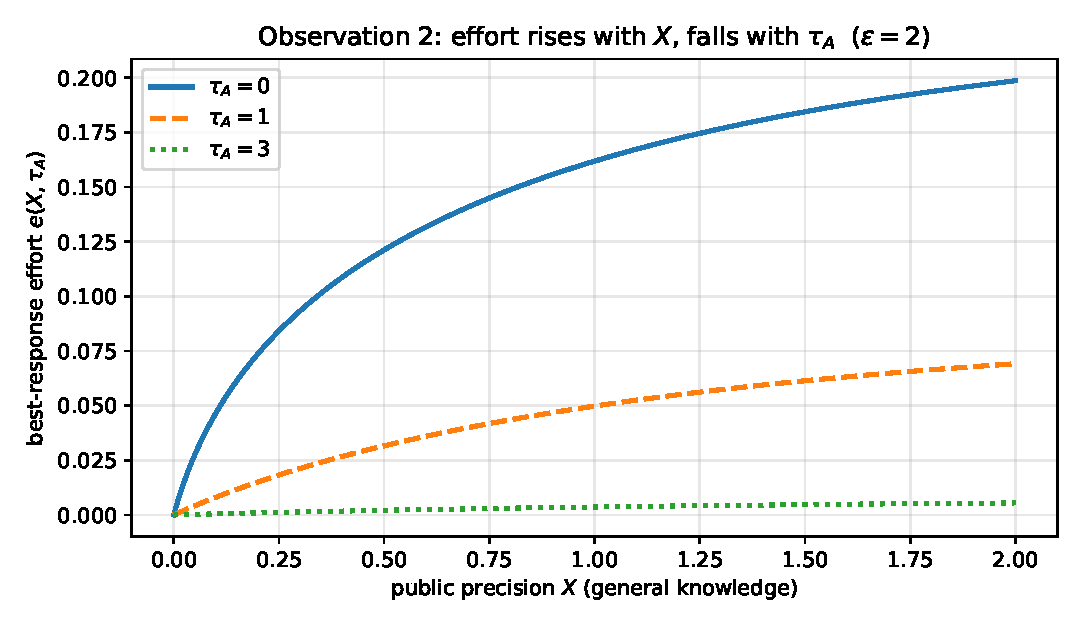
\includegraphics[height=0.78\textheight]{analysis/figures/best_response.pdf}
  \end{center}
\end{frame}

\begin{frame}{B2 \textperiodcentered{} Transition map $F$, $\varepsilon=2<4$: a unique positive steady state}
  \begin{center}
    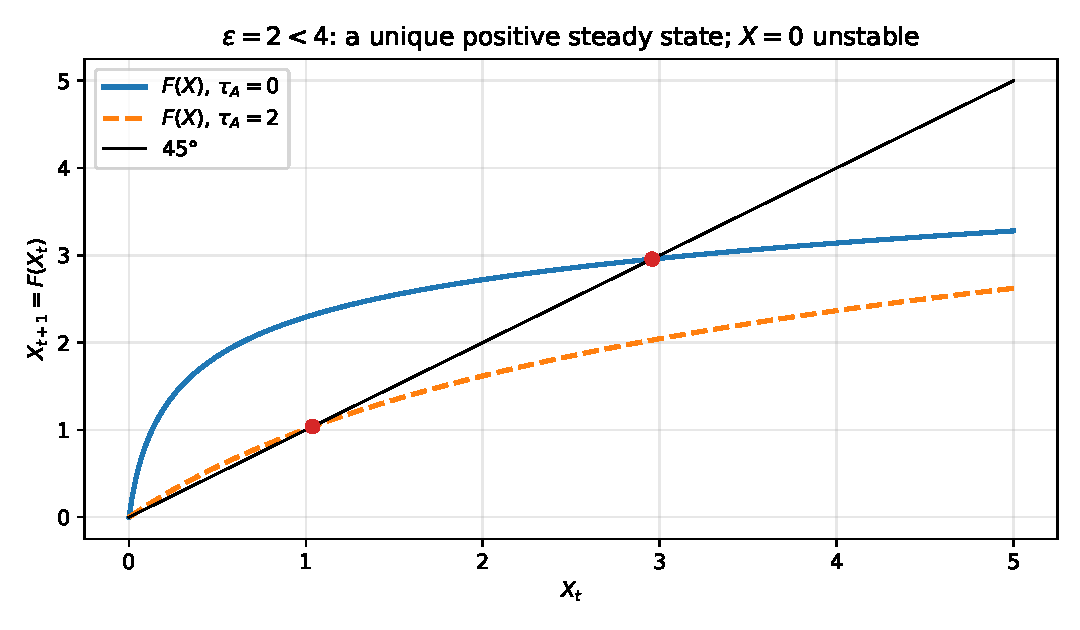
\includegraphics[height=0.78\textheight]{analysis/figures/transition_eps2.pdf}
  \end{center}
\end{frame}

\begin{frame}{B3 \textperiodcentered{} Transition map $F$, $\varepsilon=6>4$: three steady states, then complete collapse}
  \begin{center}
    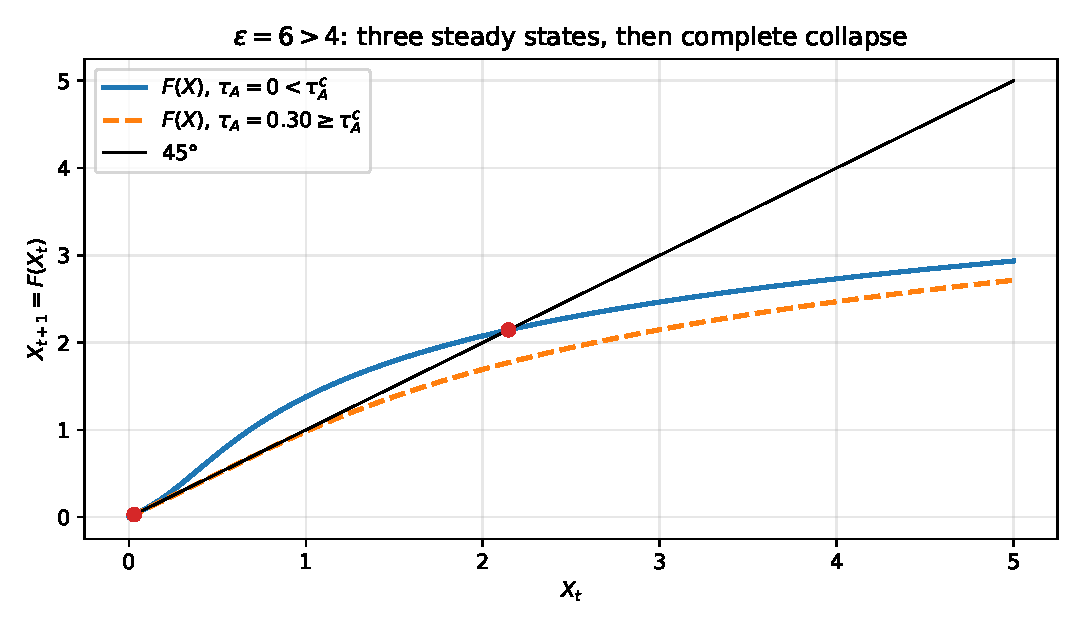
\includegraphics[height=0.78\textheight]{analysis/figures/transition_eps6.pdf}
  \end{center}
\end{frame}

\begin{frame}{B4 \textperiodcentered{} Steady-state welfare against $\tau_A$, $\varepsilon=2$: single-peaked}
  \begin{center}
    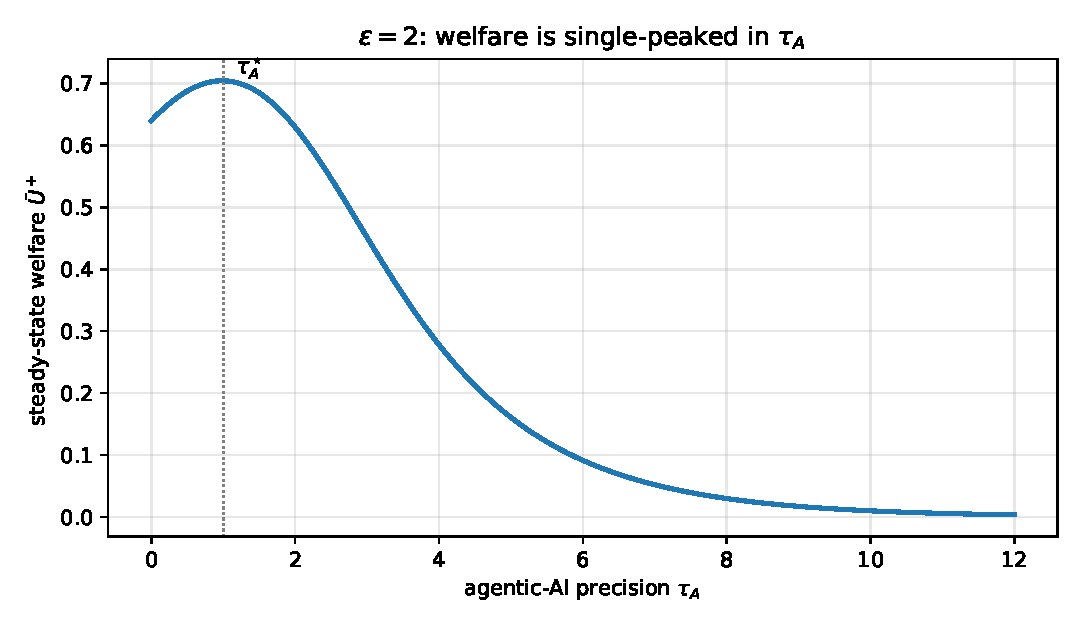
\includegraphics[height=0.78\textheight]{analysis/figures/welfare_eps2.pdf}
  \end{center}
\end{frame}

\begin{frame}{B5 \textperiodcentered{} Steady-state welfare against $\tau_A$, $\varepsilon=6$: a cliff at $\tau_A^c$}
  \begin{center}
    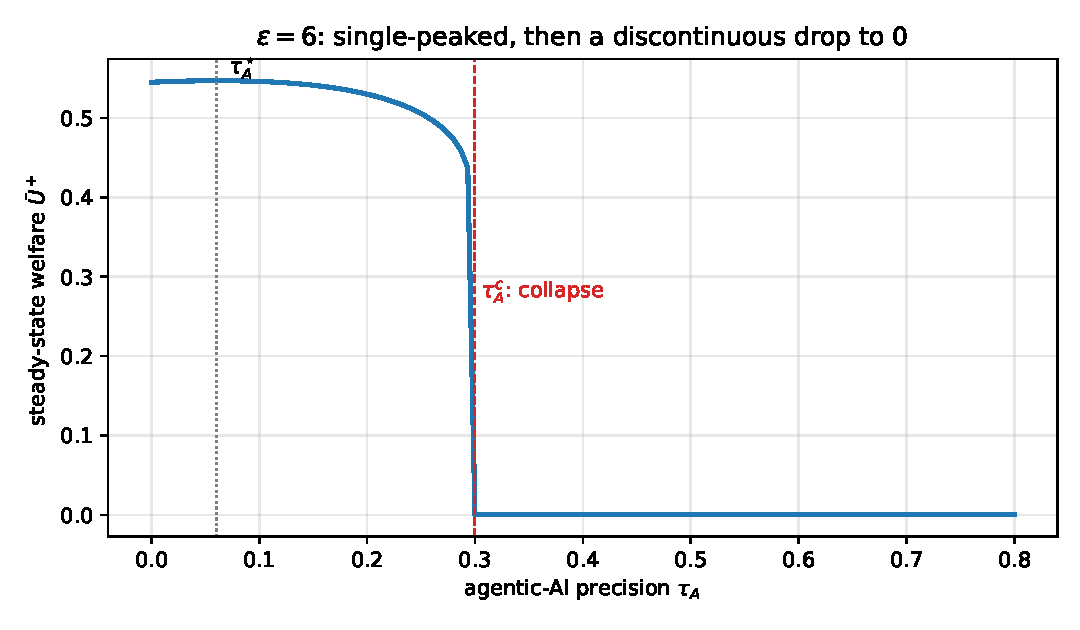
\includegraphics[height=0.78\textheight]{analysis/figures/welfare_eps6.pdf}
  \end{center}
\end{frame}

%================= BACKUP: LEAN =======================================
\begin{frame}[fragile]{B6 \textperiodcentered{} Lean I: Observation 1 as a statement about a derivative}
  \small\textbf{Paper claim.} $\partial^2U/\partial e\partial X=\Delta_X\lambda_I g(X)g(Y)>0$.
  \textbf{Spec} (\texttt{PaperInterface.lean}; $G,g$ abstract with $G'=g$, $g>0$):
\begin{lstlisting}
def paper_observation_1_complementSpec : Prop :=
  ∀ (ΔX lamI p0 τ e X ε : ℝ) (G g : ℝ → ℝ),
    0 < ΔX → 0 < lamI → HasDerivAt G (g X) X → 0 < g X → 0 < g (p0 + lamI * e + τ) →
      HasDerivAt (fun X' : ℝ => ΔX * G X' * lamI * g (p0 + lamI * e + τ) - e ^ (1 / ε))
          (ΔX * lamI * g X * g (p0 + lamI * e + τ)) X
        ∧ 0 < ΔX * lamI * g X * g (p0 + lamI * e + τ)
\end{lstlisting}
  \textbf{Proof} (\texttt{ProofInterface.lean}): the chain rule, then the sign.
\begin{lstlisting}
theorem paper_observation_1_complement : paper_observation_1_complementSpec := by
  intro ΔX lamI p0 τ e X ε G g hΔ hlam hG hgX hgY
  refine ⟨?_, ?_⟩
  · have h := (((hG.const_mul ΔX).mul_const lamI).mul_const (g (p0 + lamI * e + τ))).sub_const
      (e ^ (1 / ε))
    exact h.congr_deriv (by ring)
  · exact mul_pos (mul_pos (mul_pos hΔ hlam) hgX) hgY
\end{lstlisting}
  \textbf{Reading.} \texttt{HasDerivAt} states the derivative of the marginal utility in $X$; \texttt{mul\_pos} certifies
  the sign. The substitute part is identical with $g'(Y)<0$ and \texttt{mul\_neg\_of\_pos\_of\_neg}.
\end{frame}

\begin{frame}[fragile]{B7 \textperiodcentered{} Lean II: the FOC as a real derivative, and Observation 2 without Topkis}
  \small\textbf{FOC.} Lean differentiates (6) in $e$ --- \texttt{Real.hasDerivAt\_rpow\_const} for the cost, the chain rule for $G(Y)$:
\begin{lstlisting}
def paper_first_order_conditionSpec : Prop :=
  ∀ (f00 ΔG ΔX p0 lamI τ X ε e : ℝ) (G g : ℝ → ℝ),
    0 < e → 0 < ε → HasDerivAt G (g (p0 + lamI * e + τ)) (p0 + lamI * e + τ) →
      HasDerivAt (fun e' : ℝ => f00 + G X * ΔG + G X * G (p0 + lamI * e' + τ) * ΔX
          - ε / (ε + 1) * e' ^ ((ε + 1) / ε))
        (ΔX * G X * lamI * g (p0 + lamI * e + τ) - e ^ (1 / ε)) e
\end{lstlisting}
  \textbf{Observation 2 in $X$}, stated as a comparison of two FOC solutions ($g$ decreasing and positive on $[\sigma^{-2},\infty)$):
\begin{lstlisting}
def paper_observation_2_increasing_in_XSpec : Prop :=
  ∀ (ΔX lamI p0 τ ε GX1 GX2 e1 e2 : ℝ) (g : ℝ → ℝ),
    0 < ΔX → 0 < lamI → 0 < ε → 0 < p0 → 0 ≤ τ →
    AntitoneOn g (Set.Ici p0) → (∀ y ∈ Set.Ici p0, 0 < g y) →
    0 ≤ GX1 → GX1 < GX2 → 0 ≤ e1 → 0 ≤ e2 →
    ΔX * GX1 * lamI * g (p0 + lamI * e1 + τ) = e1 ^ (1 / ε) →
    ΔX * GX2 * lamI * g (p0 + lamI * e2 + τ) = e2 ^ (1 / ε) →
      e1 < e2
\end{lstlisting}
  \textbf{Proof idea.} If $e_2\le e_1$ the benefit at $(e_2,X_2)$ exceeds $e_1^{1/\varepsilon}\ge e_2^{1/\varepsilon}$: contradiction.
\end{frame}

\begin{frame}[fragile]{B8 \textperiodcentered{} Lean III: Lemma 1, Proposition 2, and the two things Lean pushed back on}
  \small\textbf{One lemma carries Lemma 1 and Proposition 2:} $A\mapsto(\Sigma^2+A^{-1})^{-1}$ is strictly increasing on positives.
\begin{lstlisting}
def paper_lemma_1_transition_strictly_increasingSpec : Prop :=
  ∀ (Sig2 lamG I : ℝ) (e : ℝ → ℝ),
    0 < Sig2 → 0 < lamG → 0 < I → MonotoneOn e (Set.Ici 0) → (∀ X, 0 ≤ e X) →
      StrictMonoOn (fun X : ℝ => (Sig2 + (X + lamG * I * e X)⁻¹)⁻¹) (Set.Ioi 0)
\end{lstlisting}
  \textbf{Boundary.} Lean's $0^{-1}=0$: the paper's $F(0)=0$ is a limit convention, so the rows live on $X>0$:
\begin{lstlisting}
theorem transition_at_zero_lean_convention (Sig2 lamG I : ℝ) :
    (Sig2 + ((0 : ℝ) + lamG * I * 0)⁻¹)⁻¹ = Sig2⁻¹ := by simp
\end{lstlisting}
  \textbf{The untouched assumption.} With $\Delta_I>0$ the marginal benefit of effort at $X=0$ is positive
  (and, by \texttt{transition\_positive\_with\_effort}, $F(0)>0$):
\begin{lstlisting}
theorem effort_incentive_survives_without_general_knowledge (ΔI ΔX lamI p0 τ : ℝ) (g : ℝ → ℝ)
    (hΔI : 0 < ΔI) (hlam : 0 < lamI) (hg : 0 < g (p0 + τ)) :
    0 < ΔI * lamI * g (p0 + τ) + ΔX * 0 * lamI * g (p0 + τ)
\end{lstlisting}
  \textbf{What Lean verifies.} 13/13 rows closed; \texttt{lake build}: success (4000 jobs); \texttt{check --fast}: exit 0.
  Not derived: the Gaussian facts $G'=g$, $g'<0$ --- hypotheses, the declared boundary.
\end{frame}

%================= BACKUP: TRAMPA Y VERSIONES ==========================
\begin{frame}{B9 \textperiodcentered{} This week's trap: welfare, and the assumption Section 5 never relaxes}
  \footnotesize
  \begin{columns}[T]
    \column{0.5\textwidth}
      \textbf{Is welfare increasing in AI accuracy?} No.
      \begin{itemize}
        \item $\varepsilon<4$ + Assumption 2: $\bar U^+$ strictly increasing on $(0,\tau_A^\star)$, strictly
          decreasing after, $\to 0$ (Prop.\ 10).
        \item $\varepsilon>4$: same up to $\tau_A^c$, then $\bar U^+=0$ (Prop.\ 11); also the basin threshold
          $\bar X_m$ rises with $\tau_A$ (Prop.\ 7).
        \item Scaling law: $\tau_A^c/\log I\to 2/\varepsilon$, $\tau_A^\star/\log I\to 2/(\varepsilon+1)$
          (Prop.\ 12); without Assumption 2 the profile need not be single-peaked (footnote 8).
      \end{itemize}
      \textbf{Why the intuition fails:} effort is under-supplied (externality); a better AI lowers effort
      (Obs.\ 2), which lowers $\bar X_h$ (Prop.\ 2, 4, 8); the indirect loss grows with $\tau_A$ while the
      direct gain has diminishing returns ($g$ falls).
    \column{0.5\textwidth}
      \textbf{Assumptions the authors relax (Section 5).}
      \begin{tabular}{@{}p{2.5cm}p{4.2cm}@{}}
        \toprule
        5.1 Aggregation & $I(\tau_A)=I_0+e^{\eta\tau_A}$; results survive if $\eta<\varepsilon/2$ (Prop.\ 14) \\
        5.2 Synthetic data & $\tau_{syn}>0$ puts a floor under $X$ (Prop.\ 15) \\
        5.3 Separability & public signal $\propto e^\beta$; threshold $\varepsilon<4/\beta$ (Prop.\ 16) \\
        \bottomrule
      \end{tabular}

      \smallskip
      \textbf{Never touched:} Assumption 1's $\Delta_I=0$ --- context-specific knowledge has \emph{zero} standalone
      value. It is a production-function assumption (page 9), and it is what makes the private return to effort
      vanish with $X$, what makes $(\bar X,\bar e)=(0,0)$ a steady state, and what gives the collapse state
      welfare $0$ (Section 4.1). With $\Delta_I>0$: effort at $X=0$ is $\Delta_I\lambda_I g(\sigma^{-2}+\tau_A)>0$,
      $F(0)>0$, no collapse fixed point (Lean, B8). Also untouched: the additive precision in (4), i.e.\ AI and
      own learning as perfect substitutes for context.
  \end{columns}
\end{frame}

\end{document}
